\documentclass{beamer}
\usepackage{siunitx}
\usepackage{tfrupee}
\let\vec\mathbf
\mode<presentation>
\usepackage{amsmath}
\usepackage{amssymb}
%\usepackage{advdate}
\usepackage{adjustbox}
%\usepackage{subcaption}
\usepackage{enumitem}
\usepackage{multicol}
\usepackage{mathtools}
\usepackage{listings}
\usepackage{url}
\usetheme{Boadilla}
\usecolortheme{lily}
\setbeamertemplate{footline}
{
  \leavevmode%
  \hbox{%
  \begin{beamercolorbox}[wd=\paperwidth,ht=2.25ex,dp=1ex,right]{author in head/foot}%
    \insertframenumber{} / \inserttotalframenumber\hspace*{2ex} 
  \end{beamercolorbox}}%
  \vskip0pt%
}
\setbeamertemplate{navigation symbols}{}
\providecommand{\nCr}[2]{\,^{#1}C_{#2}} % nCr
\providecommand{\nPr}[2]{\,^{#1}P_{#2}} % nPr
\providecommand{\mbf}{\mathbf}
\providecommand{\pr}[1]{\ensuremath{\Pr\left(#1\right)}}
\providecommand{\qfunc}[1]{\ensuremath{Q\left(#1\right)}}
\providecommand{\sbrak}[1]{\ensuremath{{}\left[#1\right]}}
\providecommand{\lsbrak}[1]{\ensuremath{{}\left[#1\right.}}
\providecommand{\rsbrak}[1]{\ensuremath{{}\left.#1\right]}}
\providecommand{\brak}[1]{\ensuremath{\left(#1\right)}}
\providecommand{\lbrak}[1]{\ensuremath{\left(#1\right.}}
\providecommand{\rbrak}[1]{\ensuremath{\left.#1\right)}}
\providecommand{\cbrak}[1]{\ensuremath{\left\{#1\right\}}}
\providecommand{\lcbrak}[1]{\ensuremath{\left\{#1\right.}}
\providecommand{\rcbrak}[1]{\ensuremath{\left.#1\right\}}}
\theoremstyle{remark}
\newtheorem{rem}{Remark}
\newcommand{\sgn}{\mathop{\mathrm{sgn}}}

\providecommand{\res}[1]{\Res\displaylimits_{#1}} 
\providecommand{\norm}[1]{\left\lVert#1\right\rVert}
\providecommand{\mtx}[1]{\mathbf{#1}}
\providecommand{\abs}[1]{\left\vert#1\right\vert}
\providecommand{\fourier}{\overset{\mathcal{F}}{ \rightleftharpoons}}
%\providecommand{\hilbert}{\overset{\mathcal{H}}{ \rightleftharpoons}}
\providecommand{\system}{\overset{\mathcal{H}}{ \longleftrightarrow}}
	%\newcommand{\solution}[2]{\textbf{Solution:}{#1}}
%\newcommand{\solution}{\noindent \textbf{Solution: }}align
\providecommand{\dec}[2]{\ensuremath{\overset{#1}{\underset{#2}{\gtrless}}}}
\newcommand{\myvec}[1]{\ensuremath{\begin{pmatrix}#1\end{pmatrix}}}

\title{Matrices in Geometry - 10.7.86}
\author{EE25BTECH11037  Divyansh}
\date{Sept, 2025}

\begin{document}

\maketitle


\section{Problem}
\begin{frame}
\frametitle{Problem Statement}
Let $\vec{C_1}$ and $\vec{C_2}$ be two circles with $\vec{C_2}$ lying inside $\vec{C_1}$. A circle $C$ lying inside $\vec{C_1}$ touches $\vec{C_1}$ internally and $\vec{C_2}$ externally. Identify the locus of center of $\vec{C}$.
\end{frame}

\section{Solution}
\begin{frame}{Solution}
Let the center of $\vec{C}$, $\vec{C_1}$ and $\vec{C_2}$ be $\vec{O}$, $\vec{O_1}$ and $\vec{O_2}$, respectively.\\
Let the radii of circles $\vec{C}$, $\vec{C_1}$ and $\vec{C_2}$ be $r$, $r_1$ and $r_2$ \\
It is given that $\vec{C}$ touches the circle $\vec{C_1}$ internally and $\vec{C_2}$ externally. Therefore, 
\begin{align}
    \norm{\vec{O} - \vec{O_1}} = r_1 - r\\
    \norm{\vec{O} - \vec{O_2}} = r_2 + r
\end{align}
Adding these two equations, we get 
\begin{align}
    \norm{\vec{O} - \vec{O_1}} + \norm{\vec{O} - \vec{O_2}} = r_1 + r_2
\end{align}
\end{frame}

\begin{frame}{Solution}
Substitute $\vec{O}$ as $\vec{x}$
\begin{align}
    \norm{\vec{x} - \vec{O_1}} + \norm{\vec{x} - \vec{O_2}} = r_1 + r_2
\end{align}
This is equation of an ellipse because it is of form 
\begin{align}
    \norm{\vec{x} - \vec{S_1}} + \norm{\vec{x} - \vec{S_2}} = 2a
\end{align}
with focii  as $\vec{O_1}$ , $\vec{O_2}$ and length of the major axis as $r_1 + r_2$
\end{frame}
\begin{frame}{Solution}
\begin{align}
    \norm{\vec{x} - \vec{O}_1} + \norm{\vec{x} - \vec{O}_2} = K, \ K=r_1+r_2
\end{align}
To eliminate square roots from the norms, we rearrange and square the equation.
\begin{align}
 \norm{\vec{x} - \vec{O}_1} = K - \norm{\vec{x} - \vec{O}_2}
\end{align}
Squaring both sides and using the property $\norm{\vec{v}}^2 = \vec{v}^{\top}\vec{v}$:
\begin{align}
 \norm{\vec{x} - \vec{O}_1}^2 = (K - \norm{\vec{x} - \vec{O}_2})^2
\end{align}
\end{frame}


\begin{frame}{Solution}
\begin{align}
    \norm{\vec{x} - \vec{O_1}} + \norm{\vec{x} - \vec{O_2}} = K, \ K=r_1+r_2
\end{align}
To eliminate square roots from the norms, we rearrange and square the equation.
\begin{align}
 \norm{\vec{x} - \vec{O_1}} = K - \norm{\vec{x} - \vec{O_2}}
\end{align}
Squaring both sides and using the property $\norm{\vec{v}}^2 = \vec{v}^{\top}\vec{v}$:
\begin{align}
 \norm{\vec{x} - \vec{O_1}}^2 = \brak{K - \norm{\vec{x} - \vec{O_2}}}^2
\end{align}
\end{frame}
\begin{frame}{Solution}
Let $S = K^2 + \norm{\vec{O_2}}^2 - \norm{\vec{O_1}}^2$ and $\vec{v} = 2\brak{\vec{O_1} - \vec{O_2}}$. The equation becomes:
\begin{align}
 2K\norm{\vec{x} - \vec{O_2}} = S + \vec{v}^{\top}\vec{x}
\end{align}
Squaring both sides again:
\begin{align}
 4K^2\norm{\vec{x} - \vec{O_2}}^2 = (S + \vec{v}^{\top}\vec{x})^2
\end{align}
\begin{align}
 4K^2\brak{\vec{x}^{\top}\vec{x} - 2\vec{O_2}^{\top}\vec{x} + \norm{\vec{O_2}}^2} = S^2 + 2S\brak{\vec{v}^{\top}\vec{x}} + \brak{\vec{v}^{\top}\vec{x}}^2
\end{align}
\end{frame}

\begin{frame}{Solution}
Using the identity $\brak{\vec{v}^{\top}\vec{x}}^2 = \vec{x}^{\top}\brak{\vec{v}\vec{v}^{\top}}\vec{x}$, we group all terms to one side to match the form $\vec{x}^{\top}V\vec{x} + 2\vec{u}^{\top}\vec{x} + f = 0$.
\begin{align}
 \vec{x}^{\top}\brak{4K^2I - \vec{v}\vec{v}^{\top}}\vec{x} + 2\brak{-4K^2\vec{O_2} - S\vec{v}}^{\top}\vec{x} + \brak{4K^2\norm{\vec{O_2}}^2 - S^2}= 0
\end{align}

\end{frame}
\begin{frame}{Solution}
    Compared with the general conic equation, we identify the matrix $V$, the vector $\vec{u}$, and the scalar $f$:
\begin{align}
    \vec{V} = 4K^2I - \vec{v}\vec{v}^{\top} = 4\brak{r_1 + r_2}^2I - 4\brak{\vec{O_1}-\vec{O_2}}\brak{\vec{O_1}-\vec{O_2}}^{\top} \\
    \vec{u} = -4K^2\vec{O_2} - S\vec{v} = -4\brak{r_1 + r_2}^2\vec{O_2} - \nonumber\\ \brak{\brak{r_1 + r_2}^2 + \norm{\vec{O_2}}^2 - \norm{\vec{O_1}}^2 }\cdot 2\brak{\vec{O_1}-\vec{O_2}} \\
    f = 4K^2\norm{\vec{O_2}}^2 - S^2 = 4\brak{r_1 + r_2}^2\norm{\vec{O_2}}^2 - \nonumber\\ \brak{\brak{r_1 + r_2}^2 + \norm{\vec{O_2}}^2 - \norm{\vec{O_1}}^2}^2
\end{align}
\end{frame}
\begin{frame}{Solution}
    \begin{figure}[H]
        \centering
        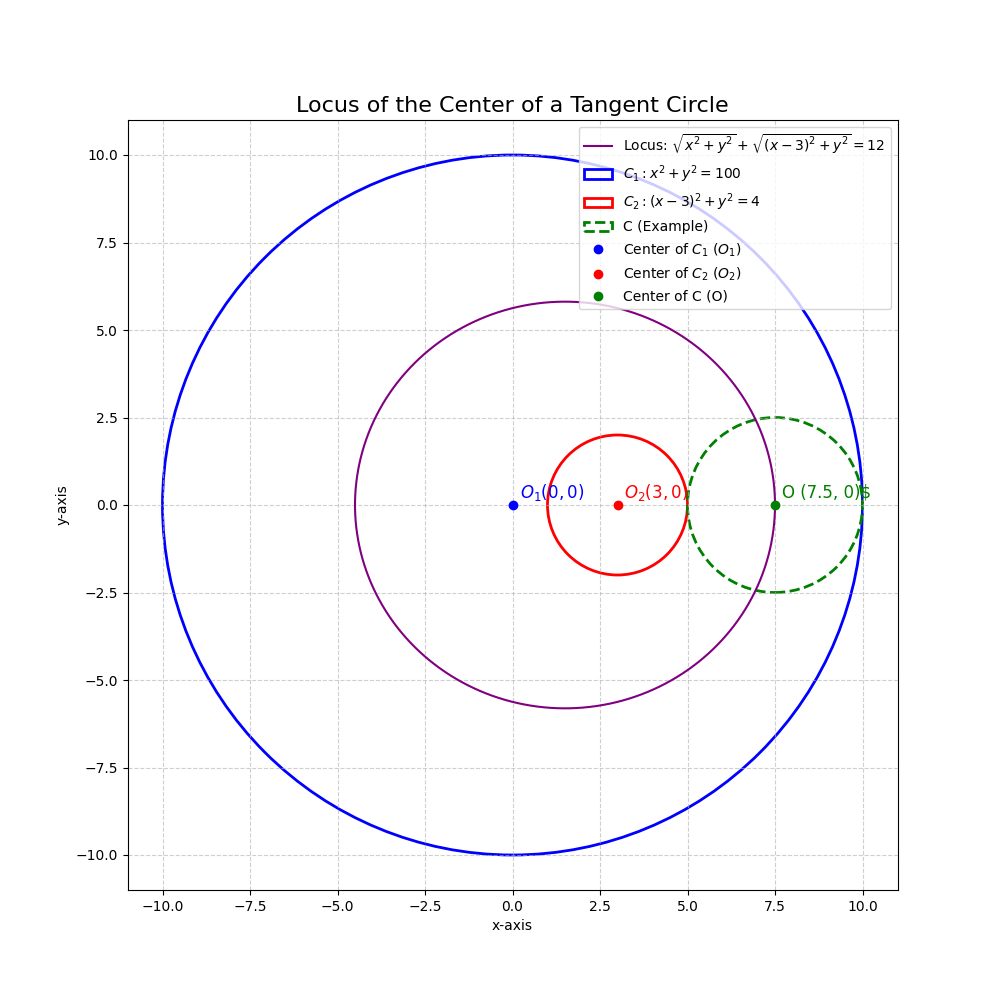
\includegraphics[width=0.5\columnwidth]{figs/1.png}
        \caption{Graph for 10.7.86}
        \label{fig:placeholder}
    \end{figure}
\end{frame}



\end{document}